% Chapter 1

% Chapter Template

\chapter{Introduction} % Main chapter title

\label{Chapter1} % Change X to a consecutive number; for referencing this chapter elsewhere, use \ref{ChapterX}

%\lhead{Chapter 1. \emph{Introduction}} % Change X to a consecutive number; this is for the header on each page - perhaps a shortened title

\renewcommand{\chaptermark}[1]{\markboth{#1}{}}
\renewcommand{\sectionmark}[1]{\markright{#1}}
\fancyhead[RE]{\small\leftmark}
% Section in the left on even pages}
\fancyhead[LO]{\small\rightmark}%Section in the left on odd pages

\section{A section goes here}

I cite something~\citet{Fuhrman2015-dynamics}
\\
A figure

\begin{figure}[h!]
	\centering
	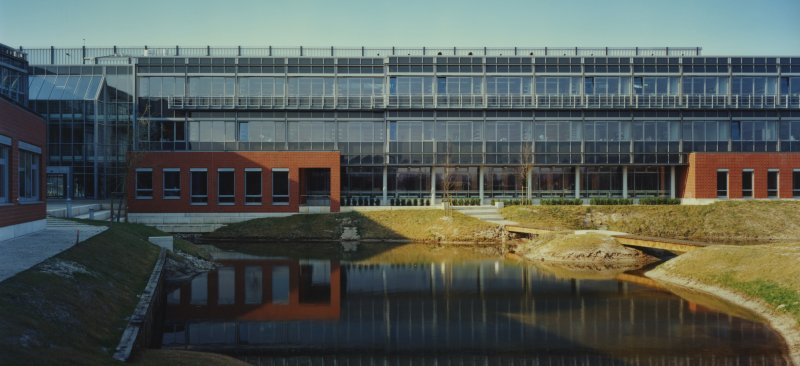
\includegraphics[width=0.6\textwidth] {Chap1_Fig1}
	\caption{\textbf{A figure example.} MMPI-MM.}\label{fig:C1Fig1}
\end{figure}

\blindmathpaper{2}
